
\chapter{Game Theory usage} \label{GAMETHEORY}
\smallskip
\hfill
\begin{minipage}[b]{8cm}
%{\it This work was presented in part at the conference of one-legged deaf-mutes in Quiberon in April 1994.}
\end{minipage}
%\begin{flushright} Remoi \end{flushright}
\vskip 2cm

{\huge I}n the automotive domain, there is a clear trend towards increased connectivity: Many new services are available today which demand a reliable communication between the car and its owner (e.g.~via smartphone applications), the manufacturer, or even the infrastructure. Many cars offer a local WiFi network and Bluetooth. Furthermore, semi-autonomous driving -- such as parking and lane keeping assistants or automatic emergency braking -- is now standard in middle to higher class models. These functionalities require a large number of sensors such as cameras, radars or other distance sensors. While these services are supposed to increase the safety of the passengers (and of pedestrians), they entail new security risks. Indeed, many attacks have been demonstrated in the recent years, some of them putting the life of the car's passengers at risk \cite{smith_car_2016}. 

The security of connected cars is taken very seriously by the manufacturers and it has become a major design goal. For instance, in a typical system architecture of a connected car, the subsystems are divided into different domains, and any message crossing a domain-border passes through a secure gateway. This allows to filter unauthorized messages and prevent an attacker who has compromised one subsystem from spreading to other -- more critical -- subsystems. However, such protections are of a \emph{static} nature. The defenses are programmed and configured once before the car leaves the factory. Because of strict certification requirements, software updates are very costly and usually must be performed by licensed workshops. This makes the relation between potential attackers and the system under attack an \emph{asymmetric} one: The attacker can analyze the car's system in order to find vulnerabilities and prepare an exploit that can then be applied -- potentially to a whole fleet of cars in parallel.   

In order to minimize the risk of such large scale attacks, it is paramount to also consider \emph{dynamic} defenses. Moving Target Defense (MTD) is a family of defense technique that proactively changes the configuration of a system in order to deceive an attacker who relies on previously gained knowledge to find and exploit vulnerabilities. MTD mechanisms may reconfigure the network, runtime environment, data, or software of the target system. Combining such mechanisms, a defense strategy based on MTD should define \emph{where}, \emph{how}, and \emph{when} to reconfigure. Critical Real-Time Embedded Systems \emph{(CRES)} -- such as connected cars or other transportation domains -- are a particularly interesting application domain for MTD: Such systems are usually used for a very long time (10+ years), and are thus exposed to the discovery of new vulnerabilities and \emph{zero-day} attacks. In addition, as CRES have limited resources (computation, communication, storage), and because their failures may have catastrophic consequences, these systems are difficult to defend using traditional methods. MTD can delay the implementation of attacks when new vulnerabilities are discovered, and limit their scope. This can be seen as a way to increase the \emph{resilience} of the attacked systems. We define resilience of a system as the capability to deliver its services in a safe way, even when faced with unknown attacks. This may be achieved by degrading certain services or by bringing the system to a safe state before critical damage has been done.   

So far, most works on MTD have focused on the question \emph{where} and \emph{how}, thus providing and evaluating new MTD mechanisms~\cite{xu_2014, taylor_automated_2016}.
Some studies have also been conducted in order to assess the efficiency of MTD in the context of risk analysis methods~\cite{hong_assessing_2016}. More recently, a few methods have been focused on the question of \emph{when} to reconfigure~\cite{lei_optimal_2017,sengupta_game_2017, feng_stackelberg_2017, li_optimal_2019, Zhang_Strat_2019}, but these contributions focus on the domain of web applications, therefore their requirements, MTD mechanisms, and models are not suitable for the design of CRES. 

Nevertheless, there exist several MTD mechanisms applicable to CRES, and for which the question \emph{how} is already answered. Instead, we focus on the questions of \emph{when} and \emph{where} to reconfigure parts of a system. 
Obviously, the question \emph{when} is actually: \emph{how often}? A question to which one may simply answer \emph{as often as possible}; but implementing an MTD mechanism has a cost, and its execution inevitably impacts the availability of the components that must be re-configured. For instance, switching IP addresses will induce communication overheads and temporary connection or packets losses. Therefore, MTD comes with an implementation cost and a quality of service (QoS) degradation.

In this paper, we aim at answering the following question: How to model MTD benefits and cost in order to find optimal MTD strategies (i.e.~\emph{where} and \emph{when} to move) in the context of CRES? We propose a combination of risk analysis techniques, MTD mechanisms, and a game-theoretic approach in order to define the best defense strategy to adopt in terms of frequency of each available MTD mechanism. 
The contributions of this paper are: 
\begin{enumerate}
    \item A game theoretic model for the defense of CRES
    \item A resolution method based on the transformation to an MILP problem
    \item A complete methodology to define the input parameters of the presented model
    \item An experimental case study for a typical connected car architecture
\end{enumerate}


\section {Motivating Example }

{\huge C}onnected cars are essentially critical and connected real-time embedded systems, that operate for an average of 15 years. 
These vehicles can be purchased by virtually anyone with a sufficient budget, including someone looking for a way to attack them. As a consequence, an attacker has time to study a specific vehicle and its defenses in order to discover vulnerabilities and ways to exploit them. 
An attacker who owns a vehicle can also use this vehicle to gain access to the manufacturer's network in order to mount remote attacks on vehicles on the same network. This could eventually allow to infect an entire fleet.

Regarding the security of connected cars, software updates are difficult to perform on these widely distributed systems with limited computation and communication capacities.
This means that car manufacturers must mainly rely on defenses deployed when the vehicle is sold or updated. 
The asymmetry between attackers and defenders is therefore very significant in the context of connected cars. 

\begin{figure}[h]
    \centering
    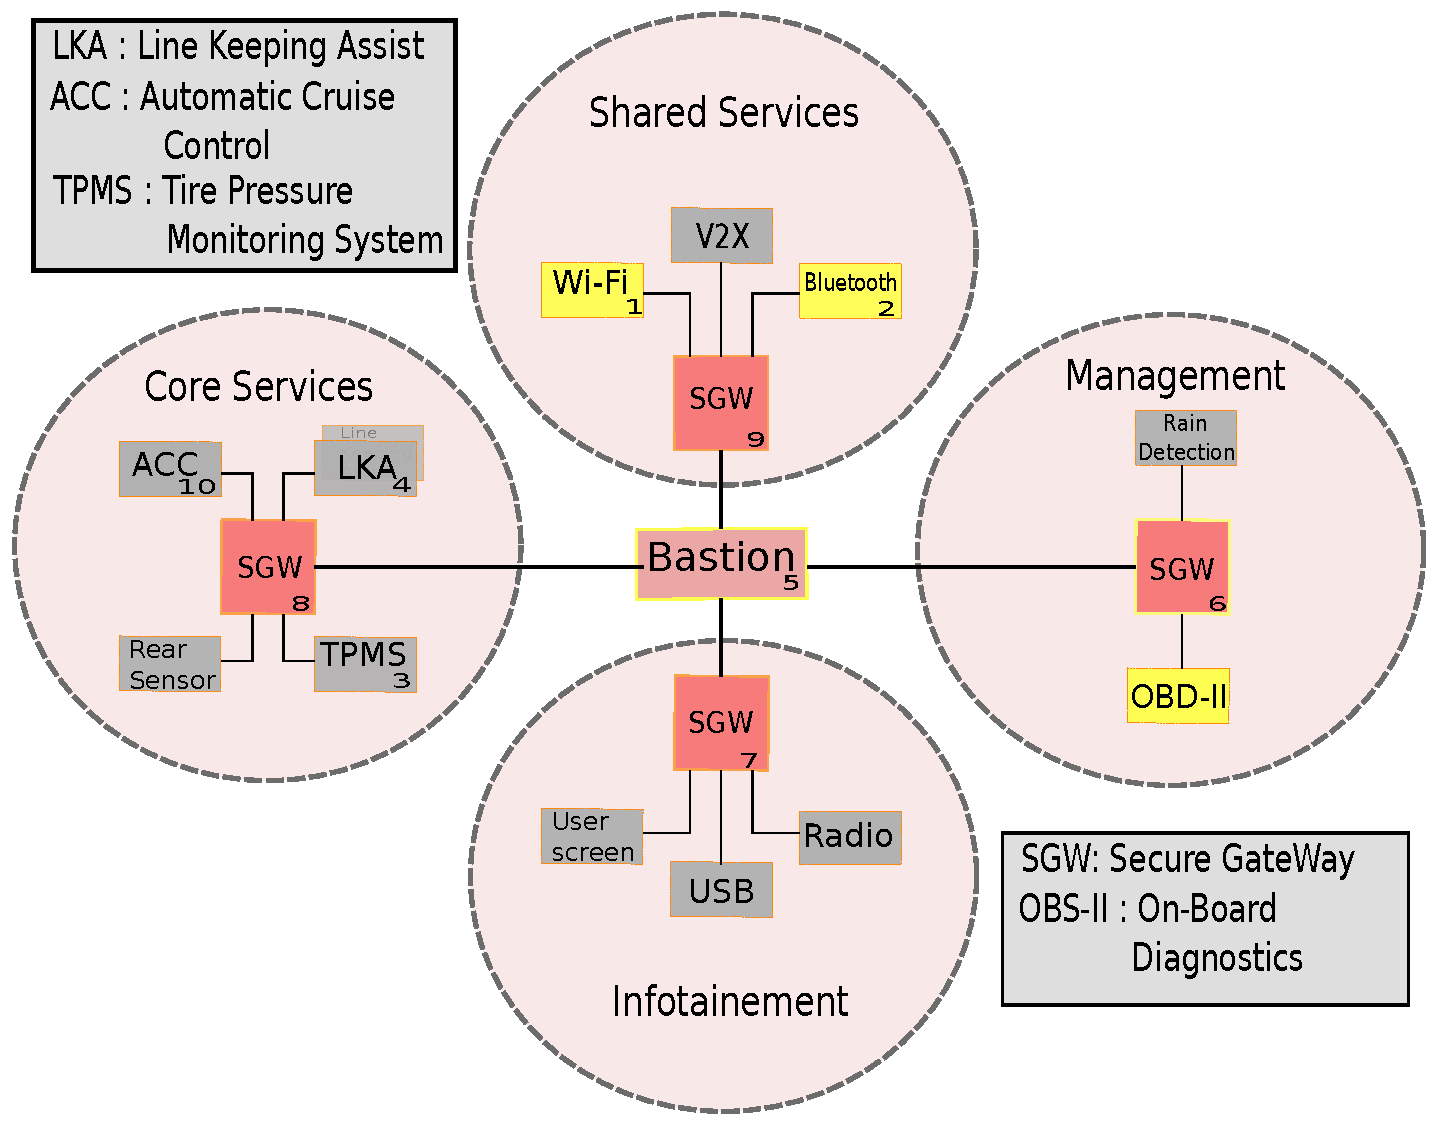
\includegraphics[width=0.7\textwidth]{schema/car_architeccture_compact.pdf}
    \caption{Vehicle Architecture scheme}
    \label{fig:game_archi}
\end{figure}

An example of the internal architecture of a connected car is presented in Figure~\ref{fig:game_archi}. This type of architecture is called \textit{architecture by domain} because the different services of the vehicle are separated into four domains according to their role:

\begin{enumerate}
    \item \textbf{Infotainment}: services related to the user experience such as the radio, the on-board screen, and various applications accessible to the user. 
    \item \textbf{Core Services}: critical services for the operation of the vehicle such as cruise control, brake controls, or lane keeping assistant.
    \item \textbf{Management}: services dedicated to diagnostics and updates of the vehicle, such as the OBD-II \textit{(On-Board Diagnostic)} plug. 
    \item \textbf{Shared Services}: regroups services allowing to communicate with the outside world (V2X) as well as some services shared among several domains.
\end{enumerate}

Within each of these domains, the communication is managed by a Secure Gateway serving as router and firewall. For example, in the Infotainment domain, if the USB module wants to send a message to the user screen module, those messages must go through the domain's Secure Gateway.

All the communication between two separate domains must pass through an entity called the \textit{Bastion}, operating as a \textit{"super" Secure Gateway}. If the Bluetooth module located on the Shared services domain wants to communicate with the user screen module located on the Infotainment domain, all the messages will be examined and filtered by the Bastion.
The \textit{Bastion} is basically a router and a firewall for the communication between the domains. Typically, it also embeds an IDS \textit{(Intrusion Detection System)} in order to detect any attempt of intrusion into the vehicle's system.

This architecture has been designed with safety and security in mind, and the vehicle already possesses some defenses located on the secure gateways. But these defenses are static, i.e.~they have a configuration that will remain the same throughout the entire life cycle of the vehicle. If an attacker finds a vulnerability and a way to bypass an existing defense, the attack has a high chance of being reproducible and may be applied to any number of vehicles of the same type. 

Consider as an example the access code to the vehicle's Bluetooth module -- providing an entry point for attackers that target the vehicles integrity -- and the Bluetooth MAC address, which is of interest for attackers that aim to compromise the driver's privacy (e.g.~by tracking the vehicle).
The Bluetooth access key is generated only once, allowing a trusted device to access the Bluetooth module. 
It is relatively easy for an attacker to retrieve the access key of this module. The attacker will then be able to use the recovered key to connect to the Bluetooth module and gain access to the CAN bus of the vehicle in order to send forged messages, potentially compromising the integrity of the vehicle.
The MAC address of the Bluetooth module is visible in clear to all nearby peripherals. Once the correspondence is made between the MAC address and the associated vehicle, it is possible to follow the comings and goings of this vehicle in the areas monitored by an attacker. 
 
The introduction of MTD on the Bluetooth module can help to limit such attacks, and thus to slow down the progression of an attacker.
For example, we can periodically change the access code to the Bluetooth module. By using a period smaller than the time necessary for an attacker to discover the access code, it becomes harder for an attacker to succeed in connecting to the vehicle's Bluetooth module.
Similarly, by periodically changing the MAC address of the vehicle's Bluetooth module, it becomes more onerous for an attacker to maintain a correspondence between a MAC address and a vehicle, making it more difficult to track. 

However, there is a drawback of using MTD in a connected vehicle. Indeed, connected vehicles are critical embedded systems with limited computing power and strong time and QoS constraints.
The use of MTD on a vehicle will have an impact on these three elements. It is therefore necessary to find a good balance between the protection of the vehicle and the operating constraints related to this type of system.
Therefore, we are interested in finding the best strategy for using the different MTD in the vehicle and thus be able to determine the frequency of use of each MTD on each asset, allowing the vehicle to be as well protected as possible against all types of existing and future attacks. 
As a solution to this problem, we propose a model representing the interactions between a set of attackers and a connected vehicle, as well as all the constraints that the system must respect.


\section {Model presentation}

{\huge I}n this section, we present our model, starting with the basic structure, and discussing the different input parameters in the following.

\subsection{Model Structure}

\label{game_struct}

The game we use will be represented by the tuple $<N, (M_i)_{i \in N}, P, R_{nmpn'm'}, \widehat{R}_{nmpn'm'}>$ in which: 

\begin{itemize}
	\item $N = \{0, 1,...,n\}$ : the set of nodes of the system under attack. 
	\item $M_i = \{0,1,..,m_i\}$ : the set of MTD defenses present on node $i$. 
	\item $P = \{0, 1,...,p\}$ : the set of attacker profiles.
	\item $R_{nmpn'm'}$ : reward obtained by the defender when he chooses to use the MTD $m$ on node $n$ while the attacker $p$ targets the MTD $m'$ on node $n'$.
	\item $\widehat{R}_{nmpn'm'}$ : reward obtained by the attacker $p$ when she chooses to use to target the MTD $m'$ on the node $n'$ while the defender will defend the node $n$ with the MTD $m$. \\
\end{itemize}


The game is composed of a set of nodes $N$ corresponding to the elements present in each domain, such as the SGW, the Bluetooth, or the ACC.
On each of these nodes, a set of assets is present, corresponding to  valuable information or subsystems. 
Each of these assets is protected by one or several MTDs of the set $M_i$.
The different attackers are represented by the set of attacker profiles $P$, each of which has the objective to target some assets present on the different nodes, depending on the profile type.

Resolving the game consists in finding the best defense strategy for the defender against the set of attacker profiles taken into account.
The decision variables of the problem corresponding to the strategies chosen by the two players and are represented as follows:

\begin{itemize}
	\item $\delta_{nm}$: The strategy of the defender on the node $n$ and its MTD $m$.
	\item $\alpha_{pn'm'}$: The strategy of the attacker of profile $p$ on the MTD $m'$ of node $n'$.
\end{itemize}

%On each node of the studied system there is potentially one or more assets that we want to hide from an attacker.
%In our game, we represent each node having at least one information to hide by a node. Knowing that each information can be protected by one or more MTD.

On each node, the defender has a budget of $1$ to spend. The distribution of this budget corresponds to the frequency of use of each MTD over a period of time and will be represented the decision variable $\delta_{nm}$.

Each attacker has a global budget of $1$ to spend on the whole game, and will choose only one node to target. As we will consider several types of attackers, each with different objectives to achieve, they will not necessarily all be interested in all the assets present on a node. 

\begin{figure}[h]
    \centering
    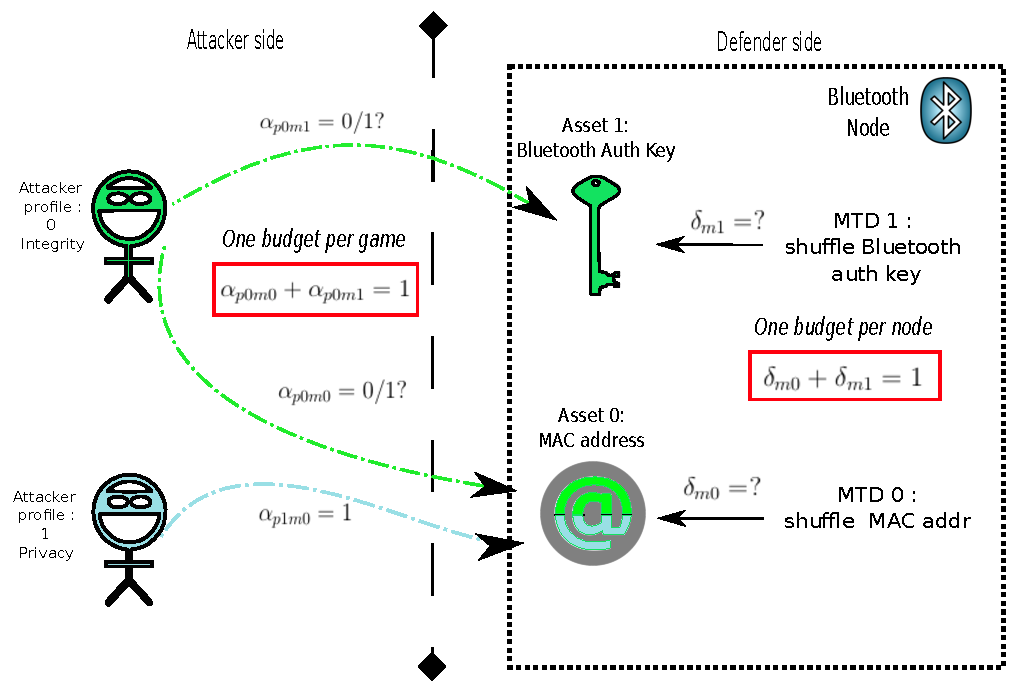
\includegraphics[width=0.95\textwidth]{schema/node_archi_3.pdf}
    \caption{Model Representation for one node and 2 attacker profiles}
    \label{fig:node_pres}
\end{figure}

To illustrate our model, Figure~\ref{fig:node_pres} shows a game composed of one node with two assets to protect and two MTD, as well as two attackers of different types.
The attacker of profile $0$ is interested in recovering the authentication key of the Bluetooth module as well as the MAC address of the module.
The attacker of profile $1$ is only interested in the MAC address of the Bluetooth module. Therefore, the attacker of profile $0$ will have to choose if she wants to launch an attack on the Bluetooth node via the MAC address or the Bluetooth key. The attacker of profile $1$ will always choose to attack the node via the MAC address because it is the only information she is interested in on this node. 

The defender needs to decide how to use the two available MTD in the most efficient way knowing what the attackers are interested in. The resolution of the game will allow us to determine the optimal strategy of using the MTD, allowing to defend the system in the best possible way against the different attackers.

\subsection{Input Parameters}

Before defining the reward functions associated to each couple of attacker-defender actions, we begin by identifying the different input parameters of the game.
These parameters must determined in order to instantiate the model for a specific use case. 

The following parameters describe the attacker side:\\

\begin{table}[h]
\begin{tabular}{ll}
\multicolumn{1}{l}{$\widehat{Sp}_{nmp}$} & \multicolumn{1}{l}{Success probability of attacker profile $p$ on node $n$ when MTD $m$ is used.}     \\ 
\multicolumn{1}{l}{$\widehat{W}_{np}$}   & \multicolumn{1}{l}{Attacker profile $p$ interest in the node $n$.}                                             \\
\multicolumn{1}{l}{$\widehat{C}_{nmp}$}  & \multicolumn{1}{l}{Cost for the attacker of type $p$ to attack MTD $m$ on node $n$.} \\ 
\multicolumn{1}{l}{$\widehat{\gamma}_p$} & \multicolumn{1}{l}{Probability to encounter attacker profile $p$.}                                          \\ 
\end{tabular}
\end{table}

The following parameters describe the defender side:\\

\begin{table}[h]
\begin{tabular}{ll}
\multicolumn{1}{l}{$W_{np}$}             & \multicolumn{1}{l}{Defender interest on node $n$ when the attacker profile $p$ targets it.}                         \\ 
\multicolumn{1}{l }{$C^{MTD}_{nm}$}       & \multicolumn{1}{l}{Defender cost to use the MTD $m$ on node $n$.}                                           \\ 
 \end{tabular}
\end{table}


%The methodology to characterize the values related to all of these parameters will be seen  in the next subsection~\ref{methodo}.

\subsection{How to Determine the Parameters}
\label{param-method}

To realistically define a model, we need to characterize the parameters of the game in order to define them correctly.
We assume that the following information are known:

\begin{itemize}
	\item The entropy value associated to each element that we want to protect by an MTD. This corresponds e.g.~to the number of valid IP addresses that can be used or the number of MAC addresses available for an element.
	\item The CVSS score associated with each asset of the system we are considering in the game. This will allow us to know the interest that one of the players may have in this node, the more vulnerable it is, the more it may interest an attacker. This score is computed by taking in account the difficulty to access a specific resource and the requirements to launch an attack.
	\item For each MTD, the time during which the corresponding service is not accessible if the defense is used.
	\item For each attacker profile and information to protect, the time needed for an attacker to scan an occurrence of the information.
	\item For each node, the associated reconfiguration period.
\end{itemize}

In the following, we will detail different methods used to determine the input parameters defined in the previous section.

\label{methodo}

\subsubsection{Success Probability: $\widehat{Sp}_{nmp}$}

We start by defining the success probability of an attacker for a given MTD and node.

First of all, when an attacker of profile $p$ is not interested in the asset or information protected by MTD $m$ on node $n$, we fix the corresponding success probability to $0$ in order to incite the attacker not to target this asset.
If the attacker is indeed interested in an asset or information; there are several ways to determine the value of the success probability:

\begin{enumerate}
	\item When the MTD $m$ used is of type shuffle, we apply the \textit{urn statistical model}~\cite{carroll_analysis_2014}, to solve the problem of \textit{Drawing with Replacement}. In our case, the number of attempt is equal to the node period divided by the time needed to scan one configuration. The formulation of this problem is given by the equation~\eqref{proba}, where $x$ is the number of attempts, $h$ is the number of instances of the asset, $a$ the number of available values. The probability to find the information can then be calculated as
	\begin{flalign} &\widehat{Sp} = 1 - ((a-h)/a)^x \label{proba}\end{flalign}
    \item When the MTD $m$ is not of shuffle type, and a method to bypass this MTD exists, the attacker's success probability is equal to the duration of the reconfiguration period of the node $n$ divided by the time to bypass the MTD. If the duration of a period is greater, the attacker's success probability is equal to $1$.
	\item When the MTD $m$ used is neither of type shuffle, nor has a method to bypass, we will need to resort to an adhoc method to estimate the success probability.\\[1ex]
\end{enumerate} 


\noindent\textbf{Example: } 
Consider an attacker trying to find the IP address of a module on an IPV4 sub-network. On this particular sub-network 252 addresses are valid and usable by a module.

In order to estimate the time an attacker needs to scan the network, we consider a well-known open source tool for scanning networks: nmap. In fact, nmap can be used to discover hosts and services
on a network by sending packets and analyzing the responses. It can also provide further information on targets (e.g.~reverse DNS names, device types, MAC addresses, etc.). Using nmap with highly optimized options, the time needed to scan one IP address is approximately 255 ms~\cite{nmap}.

Considering that the defender can change the IP address of the module sought by the attacker every 10 seconds, the attacker will have $10/0.255 = 39,21$ attempts to find the correct address.
Assuming that the module is the only element present on the network, according to formula~\eqref{proba}, the attacker's probability of success in discovering the IP address of the module is

\begin{flalign*} 
&\widehat{Sp} = 1 - ((a-h)/a)^x \\
&\widehat{Sp} = 1 - ((252-1)/252)^{39} \\
&\widehat{Sp} = 1 - 0,856355413 =  0,143644587
\label{proba2}\end{flalign*}

\subsubsection{Attacker Gain: $\widehat{W}_{np}$}
%% Interest --> Gain? Profit?

The interest of an attacker of profile $p$ for a node $n$ will depend on the type of information contained on this node.
If there is at least one piece of information on node $n$ that could be of interest to the attacker, the value of the attacker's interest $p$ for this node will be equal to the corresponding CVSS score. The higher the CVSS score for a node's asset, the easier and more interesting it will be for an attacker to launch an attack on it.
If on the other hand none of the information of node $n$ is of interest to the attacker $p$, the interest of the attacker $p$ for this node will be equal to 0.

 \subsubsection{Attack Cost: $\widehat{C}_{nmp}$}

The definition of the cost related to an attack depends on the type of MTD $m$ used on the node $n$. 
If this one corresponds to a shuffle MTD, the cost of an attack will be equal to the cost of launching a scan multiplied by the number of scans that can be performed during the reconfiguration period of the node.
If the MTD used does not correspond to a shuffle type MTD, the cost will correspond to the cost of using the MTD bypass method.

\subsubsection{Attacker Appearance Probability: $\widehat{\gamma}_p$}

The definition of the probability of appearance of an attacker can be done in two ways. If we have access to the history of different attacks that have already taken place on the same type of system, it is possible to extract the probability of occurrence of an attacker profile. Obtaining this kind of information is difficult, since car manufacturers typically so not share such information with the public.

Therefore, if this type of history is not available or does not exist, we propose to use an exponential distribution, depending on the level of expertise of the attacker. This reflects the fact that there are many  beginners, some serious attackers and very few experts.

% FIXME: Give the formula to calculate the normalized probabilities, given parameter \lambda

\subsubsection{Defender Node Gain: $W_{np}$}
%% EB: Interest --> Profit? Gain?
The interest of a node for the defender to defend against an attacker $p$ will depend on the node $n$ as well as the information contained on this node.

If none of the information on node $n$ is of interest to the profile $p$ attacker, the interest of this node for the defender will be equal to $0$. 
If at least one of these pieces of information is of interest to the profile $p$ attacker, the defender's interest in this node will be equal to the corresponding CVSS score. 
The higher the CVSS score for a node's asset, the more impact the loss of that asset will have for the defender and the greater the need for defense.

\subsubsection{MTD Usage Cost: $C^{MTD}_{nm}$}

The cost of using the MTD $m$ on node $n$ is equal to the downtime of the node induced by the use of the MTD divided by the duration of a reconfiguration period of the node.


\section {Game Formalization}

\subsection{Game Form}

{\huge A}s explained in the previous section \ref{motiv}, we have to model the problem by taking into account the interaction between several attackers and a system as well as the different constraints related to the system used.

To do this, we must first take into account the asymmetry between an attacker and the system, which is translated by the fact that an attacker will choose on which part of the system to launch an attack once she has observed the defenses used by the system.
%
We also need to consider the fact that several types of attackers are interested in the system, each with different objectives and means. The problem is that it is not possible to determine which of these attackers will appear and choose to launch an attack at which time. 

The game theoretic concepts presented in section \ref{Game_Theory} allow us to represent these different interactions and to take into account the different constraints related to the system: 
The asymmetry between the attacker and the defender gives rise to a Stackelberg game~\cite{conitzer_computing_2006} allowing to impose an order in the decision of the actions.
Bayesian games~\cite{sengupta_game_2017} allow us to represent the fact that we cannot determine the type(s) of attacker(s) to defend against and that we are looking for a strategy that will allow us to defend optimally against all the types of attackers considered.

% The use of a Bayesian Stackelberg game allows to take into account and represent the evoked characteristics between different types of attackers and a critical embedded system.


\subsection{Reward}

For each combination of actions attacker-defender on each node and MTD, a reward function allows to compute the reward corresponding to this specific combination. There is one reward function for each player. The higher the reward obtained for one action, the more the player will be interested in performing this action in the chosen context.
The computation of these reward functions is done by calculating the gain of performing the action minus the cost of performing this action.

The value of the gain of a player depends on the action of the other player. In contrast, the cost of using an action does not depend on the action taken by the other player. 

For the attacker, the gain of an action is defined as follows.
\begin{itemize}
    \item If the attacker $p$ and the defender target the same node $n$ and $n'$ and MTD $m$ and $m'$ at the same time, the associated gain for the attacker is $0$.
\item If the attacker $p$ and the defender do not target the same node $n$ and $n'$ and MTD $m$ and $m'$, the associated gain for the attacker $p$ is equal to his success probability multiplied by his interest for the node $n'$.  
\end{itemize}

The cost of performing an action for the defender corresponds to the parameter $\widehat{C}_{n'm'}$. \\

The reward function of the attacker is then of the following form: 
\begin{equation}
  \widehat{R}_{nmpn'm'} = \begin{cases}
  -\widehat{C}_{n'm'}, & \text{if } n = n' \text{ and } m = m' 
  \\
  (\widehat{Sp}_{n'm'p} * \widehat{W}_{np}) - \widehat{C}_{n'm'}, & \text{if } n \neq n' \text{ or } m \neq m'
  \end{cases}
\end{equation}
\newline

On the defender's side, the gain obtained for performing an action is defined as follows. 
\begin{itemize}
    \item If the attacker $p$ and the defender target the same node $n$ and $n'$ and MTD $m$ and $m'$ at the same time, the associated gain for the defender is equal to the probability of success of the attacker $p$ multiplied by the interest of the defender for the node.
    \item If the attacker $p$ and the defender do not target the same node $n$ and $n'$ and MTD $m$ and $m'$, the associated gain for the defender is equal to 0. 
\end{itemize}
The cost of performing an action for the defender will correspond to the parameter $C^{MTD}_{nm}$. \\

The reward function of the defender is then of the following form:
\begin{equation}
  R_{nmpn'm'} = \begin{cases}
  (\widehat{Sp}_{n'm'p} * W_{np}) - C^{MTD}_{nm}, & \text{if } n = n' \text{ and } m = m' 
  \\
  R_{nmpn'm'} =  - C^{MTD}_{nm}, & \text{if } n \neq n' \text{ or } m \neq m' 
 \end{cases} 
\end{equation}


For each pair of attacker-defender actions, on each node/MTD, the corresponding reward function must be defined. The reward functions are composed of the gain for performing an action minus the cost of performing this action. The values of the rewards will be defined according to the location targeted by the two players. The cost of an action remains the same regardless of the target chosen by the other player.
\newline

\subsection{Payoff function}

The rewards functions are used to indicate for each pair of actions and nodes, the associated rewards.
In order to determine the best possible strategy for the defender, he needs a payoff function to calculate the maximum reward he can obtain.

This function will depend on the rewards functions and on the decision variables $\alpha$ and $\delta$ representing the strategy for the attacker and the defender.

The payoff function will be the function that once maximized allows to obtain the strategy that gives the biggest possible reward to the defender.
The payoff function corresponds to the sum of all the rewards functions according to the value of the associated $\alpha$ and $\delta$ strategies and has the following form:

\begin{equation}
\sum_{n \in \mathcal{N}} \sum_{m \in \mathcal{M}} \delta_{nm} * [ \sum_{p \in \mathcal{P}} \sum_{n' \in \mathcal{N}} \sum_{m' \in \mathcal{M}} (\widehat{\gamma_p} * \alpha_{pn'm'} * R_{nmpn'm'}) - C_{nm} ]
\end{equation} 

\subsection{Complementary Slackness}

As present in section~\ref{sclack}, the complementary slackness is used to constrain each attacker to maximize her payoff function. The payoff is expressed by the following equations~\ref{game_primal}.

\begin{flalign}
&\forall_{p \in \mathcal{P}} \max_{\alpha_{np}} \sum_{n \in \mathcal{N}} [ \alpha_{np} [ \sum_{m \in \mathcal{M}} \delta_{nm}^{} (\widehat{R}_{nmp}^{} - \widehat{C}_{nmp}) + \delta_{nd}^{}(\widehat{R}_{ndp}^{} - \widehat{C}_{ndp}) ] ] \nonumber \\ 
&\forall_{p \in \mathcal{P}} \sum_{n \in \mathcal{N}} \alpha_{np} = 1 \nonumber\\
&\forall_{p \in \mathcal{P}} \forall_{n \in \mathcal{N}} \alpha_{np} \geq 0 
\label{game_primal}
 \end{flalign}

It is then possible to transform the primal problem~\ref{game_primal} into its dual~\ref{game_dual}. 
Here, the function aims at finding for each profile $p$ the smallest value of the variable $a_p$ that will be equal to the maximum reward that the attacker $p$ can obtain given the strategy chosen by the defender.

\begin{flalign}
&\forall_{p \in \mathcal{P}} \min a_p \nonumber \\ 
&\forall{n \in \mathcal{N}}, \forall{p \in \mathcal{P}}\ a_p \geq  \sum_{m \in \mathcal{M}}  \delta_{nm}^{} (\widehat{R}_{nmp}^{} - \widehat{C}_{nmp}) \nonumber \\ &+ \delta_{nd}^{} (\widehat{R}_{ndp}^{} - \widehat{C}_{ndp}) 
\label{game_dual}
\end{flalign}

Using strong duality and complementary slackness, these two problems are  transformed into constraint (\ref{game_comple}), which must be satisfied when solving the optimization problem for the leader (defender) in order to consider only best responses by the follower (attackers).

\begin{flalign}
&\forall_{p \in \mathcal{P}} \forall_{n \in \mathcal{N}}, 0 \leq a_p - \sum_{m \in \mathcal{M}}  \delta_{nm}^{} (\widehat{R}_{nmp}^{} - \widehat{C}_{nmp}) \nonumber \\ & +  \delta_{nd}^{}(\widehat{R}_{ndp}^{} - \widehat{C}_{ndp})  \leq (1 - \alpha_{np} ) M 
\label{game_comple}
\end{flalign}

This constraint is added to the optimization problem for the defender, where $M$ is a large integer and $a_p$ is a free variable.% of the optimization problem for the defender.


\subsection{Mixed Integer Quadratic Program  (MIQP)}
\label{miqpdef}

Now that we have defined the payoff function of the defender, that we have the different parameters composing it as well as the constraints that we want the model to respect, and the formula to maximize the attackers payoff, it is possible to write the corresponding MIQP. 
This program will allow us to find the strategy $\delta$ which maximizes the reward obtained for the defender (eq.\ref{consobj}) and so to obtain the best strategy of use of the MTD present on the vehicle.

\begin{figure}[h]
\centering
  \tiny
\begin{flalign}
%\label{optim_beg}
&obj :\max_{\delta_{nm}, \alpha_{pn'm'}, a_p} \sum_{n \in \mathcal{N}} \sum_{m \in \mathcal{M}} \delta_{nm} * [ \sum_{p \in \mathcal{P}} \sum_{n' \in \mathcal{N}} \sum_{m' \in \mathcal{M}} (\widehat{\gamma_p} * \alpha_{pn'm'} * R_{nmpn'm'}) - C_{nm} ] \label{consobj}
\\ \nonumber \\
&C1 : \forall_{n \in \mathcal{N}} \sum_{m \in \mathcal{M}} \delta_{nm}^{} = 1 \label{cons1}
\\
&C2 : \forall_{p \in \mathcal{P}} \sum_{n'\in \mathcal{N}} \sum_{m'\in \mathcal{M}} \alpha_{pn'm'} = 1 \label{cons2}
 \\
&C3 :  \forall_{n' \in \mathcal{N}}  \forall_{m' \in \mathcal{M}} 0 \leq (a_p - \sum_{n \in \mathcal{N}} \sum_{m \in \mathcal{M}} \widehat{R}_{nmpn'm'} * \delta_{nm} ))   \leq (1 - \alpha_{pn'm'} ) M \label{cons3}
 \\
&\forall_{n \in \mathcal{N}} \forall_{m \in \mathcal{M}} \delta_{nm}^{} \in [0, 1] \label{cons4}
\\
&\forall_{p \in \mathcal{P}}, \forall_{n' \in \mathcal{N}} \forall_{m' \in \mathcal{M}} \alpha_{pn'm'} \in \{0,1\} \label{cons5}
 \\
&\forall_{p \in \mathcal{P}} a_p \in \mathbb{R}
\end{flalign}
\caption{MIQP representation of the game}
\label{miqp}
\end{figure}

The complete MIQP is shown in Figure~\ref{miqp}.
It is written in such a way that the defender will defend each node independently (eq.\ref{cons1}) with a budget of $1$ per node (eq.\ref{cons4}).  
It also integrates the fact that the attacker will have a budget of $1$ to spend on the whole game (eq.\ref{cons2}) and that he can choose only one target on the game (eq.\ref{cons5}).
The constraint (eq.\ref{cons3}) corresponds to the expression of the complementary slackness allowing to force each attacker to choose the target bringing him the biggest reward by taking into account the strategy of the defender. \\

Unfortunately, a MIQP is complicated to solve. In the next section we will show how we transform it into a MILP to make its resolution easier.  


\section {Game Resolution}

\label{resolution}

\subsection{MIQP to MILP Transformation}


{\huge W}e are going to transform the MIQP presented in the previous section into a MILP in order to make it easier to solve. 
To begin with, the process of transforming a MIQP into a MILP consists in going from a quadratic program with several decision variables multiplied together to a linear program in which there are no decision variables multiplied together.

To do this, we factor the two variables $\alpha$ and $\delta$ to obtain a new one named $Z$ through the following transformation: 

\begin{flalign}
& Z_{nmpn'm'} = \delta_{nm} * \alpha_{pn'm'} \label{z_transform} \\ \nonumber
\end{flalign}


Before starting to replace the $\alpha$ and $\delta$ present in the MIQP, it is necessary to make sure that it will be possible to recover their values once the MILP is solved, which will be done through the following constraints:

\begin{flalign}
& \delta_{nm} = \sum_{p \in \mathcal{P}} \sum_{n' \in \mathcal{N}} \sum_{m' \in \mathcal{M}} Z_{nmpn'm'} \label{delta_transform} \\
& \alpha_{pn'm'} = \sum_{n \in \mathcal{N}} \sum_{m \in \mathcal{M}} Z_{nmpn'm'} \label{alpha_transform}  \\ \nonumber
\end{flalign}

We will begin by transforming the objective function of the problem, by a new version containing the $Z$. We start by taking the initial function (eq. \ref{init_func}) that we have expanded into (eq . \ref{exp_func}), in order to be able to replace the values of $\alpha$ and $\delta$ present thanks to the equations (eq . \ref{z_transform}, \ref{delta_transform}) in order to obtain the new objective function of the problem (eq . \ref{new_func}).

\begin{flalign}
& \sum_{n \in \mathcal{N}} \sum_{m \in \mathcal{M}} \delta_{nm} * [ \sum_{p \in \mathcal{P}} \sum_{n' \in \mathcal{N}} \sum_{m' \in \mathcal{M}} (\widehat{\gamma_p} * \alpha_{pn'm'} * R_{nmpn'm'}) - C_{nm} ] \label{init_func} \\ \nonumber \\
& \sum_{n \in \mathcal{N}} \sum_{m \in \mathcal{M}} \sum_{p \in \mathcal{P}} \sum_{n' \in \mathcal{N}} \sum_{m' \in \mathcal{M}} [ \delta_{nm} * \widehat{\gamma_p} * \alpha_{pn'm'} * R_{nmpn'm'} ] - \sum_{n \in \mathcal{N}} \sum_{m \in \mathcal{M}} [ \delta_{nm} * C_{nm} ] \label{exp_func} \\ \nonumber \\
& \sum_{n \in \mathcal{N}} \sum_{m \in \mathcal{M}} \sum_{p \in \mathcal{P}} \sum_{n' \in \mathcal{N}} \sum_{m' \in \mathcal{M}} [ \widehat{\gamma_p} * Z_{nmpn'm'} * R_{nmpn'm'} ] \nonumber \\
&- \sum_{n \in \mathcal{N}} \sum_{m \in \mathcal{M}} [ (\sum_{p \in \mathcal{P}} \sum_{n' \in \mathcal{N}} \sum_{m' \in \mathcal{M}} Z_{nmpn'm'} ) * C_{nm} ] \label{new_func} \\ \nonumber
\end{flalign}

\subsection{Mixed Integer Linear Problem (MILP)}

The new MILP must respect the same constraints as those of the MIQP presented in section \ref{miqpdef}, adapted with the new $Z$ variables. The solution of this program must allow to obtain the same optimal strategy as the one that would have been given by the MIQP. This gives the following MILP:

\begin{flalign}
&obj :\max_{Z{nmpn'm'}, \alpha_{pn'm'}, a_p} \sum_{n \in \mathcal{N}} \sum_{m \in \mathcal{M}} \sum_{p \in \mathcal{P}} \sum_{n' \in \mathcal{N}} \sum_{m' \in \mathcal{M}} [ \widehat{\gamma_p} * Z_{nmpn'm'} * R_{nmpn'm'} ] \nonumber\\ & - \sum_{n \in \mathcal{N}} \sum_{m \in \mathcal{M}} [ (\sum_{p \in \mathcal{P}} \sum_{n' \in \mathcal{N}} \sum_{m' \in \mathcal{M}} Z_{nmpn'm'} ) * C_{nm} ] \label{obj_milp}
\\ \nonumber \\
&C1 : \forall_{n \in \mathcal{N}} \sum_{m \in \mathcal{M}} \sum_{p \in \mathcal{P}} \sum_{n' \in \mathcal{N}} \sum_{m' \in \mathcal{M}_{-idle}} Z{nmpn'm'}^{} = 1 \label{c1_milp} 
\\
&C2 : \forall_{n \in \mathcal{N}} \forall_{m \in \mathcal{M}}; 0 \leq \sum_{p \in \mathcal{P}} \sum_{n'\in \mathcal{N}} \sum_{m'\in \mathcal{M}_{- idle}} Z{nmpn'm'} \leq 1 \label{c2_milp}
\\
&C3 : \forall_{n' \in \mathcal{N}}  \forall_{m' \in \mathcal{M}} \forall_{p \in \mathcal{P}} ; \alpha_{pn'm'} = \sum_{n \in \mathcal{N}} \sum_{m \in \mathcal{M}} Z_{nmpn'm'} \label{c3_milp}
\\
&C4 :\forall_{p \in \mathcal{P}} \sum_{n' \in \mathcal{N}} \sum_{m' \in \mathcal{M}} \alpha_{pn'm'} = 1 \label{c4_milp}
\\
&C5 :  \forall_{n' \in \mathcal{N}}  \forall_{m' \in \mathcal{M}} 0 \leq (a_p - \sum_{n \in \mathcal{N}} \sum_{m \in \mathcal{M}} \widehat{R}_{nmpn'm'} * (\sum_{n" \in \mathcal{N}} \sum_{m" \in \mathcal{M}} Z{nmpn"m"} ))   \leq (1 - \alpha_{pn'm'} ) M \label{c5_milp}
\\ \nonumber \\
&\forall_{p \in \mathcal{P}}, \forall_{n \in \mathcal{N}} \forall_{m \in \mathcal{M}} \forall_{n' \in \mathcal{N}} \forall_{m' \in \mathcal{M}} Z{nmpn'm'}^{} \in [0, 1] \label{c6_milp}
\\
&\forall_{p \in \mathcal{P}}, \forall_{n' \in \mathcal{N}} \forall_{m' \in \mathcal{M}} \alpha_{pn'm'} \in \{0,1\} \label{c7_milp}
\\
&\forall_{p \in \mathcal{P}} a_p \in \mathbb{R} \label{c7_milp}
\end{flalign}


The first constraint (eq. \ref{c1_milp}) consists in limiting the defender's budget per node to $1$. 
We want to make sure with the second constraint (eq. \ref{c2_milp}) that the value that a $\delta$ can take will never exceed $1$.

Constraints 3 (eq. \ref{c3_milp}) and 4 (eq. \ref{c4_milp}) of the MILP combined together ensure that an attacker will have a budget of 1 to spend on the whole game and that the values of the different $\alpha$ can be found in the values of $Z$.

The last constraint (eq. \ref{c5_milp}) is the complementary slackness which ensures that each attacker profile will choose the node to target with the highest reward according to the strategy chosen by the defender. \\

We must now prove that this new MILP is equivalent to the initial MIQP. This will be discussed in the next subsection.

\subsection{Correspondence between the MIQP and the MILP }


In order to prove that the MILP found is indeed equivalent to the presented MIQP representing the game and its constraints, we will take all the constraints of the MIQP and show that we have their equivalent in the MILP. \\

We start with the \textbf{objective function}(eq.\ref{consobj}), whose transformation from MIQP to MILP has been presented with equation \ref{init_func},\ref{exp_func} and \ref{new_func}. This shows the equivalence between the two objective functions, showing that we are trying to solve the same problem. \\

Consider the \textbf{MIQP constraint C1} (eq.\ref{cons1}): $\forall_{n \in \mathcal{N}} \sum_{m \in \mathcal{M}} \delta_{nm} = 1$ \\
Starting from equation \ref{delta_transform}, we can replace the delta of the MIQP constraint C1(eq.\ref{cons1}) by the corresponding Z, this allows us to obtain the new constraint C1 of the MILP (eq.~\ref{c1_milp})  limiting the budget of the defender to $1$ per node. \\

We move on to the constraint \textbf{MIQP constraint C2} (eq.\ref{cons2}): $\forall_{p \in \mathcal{P}} \sum_{n'\in \mathcal{N}} \sum_{m'\in \mathcal{M}} \alpha_{pn'm'} = 1$ \\
There is the MILP constraint C4 (eq.\ref{c4_milp})  which is exactly the same as the MIQP constraint, but it does not constrain in any way the values that $Z$ can take. 
Using equation (eq.\ref{alpha_transform}), this allows us to link the values of the $\alpha$ with the one  of the corresponding $Z$, which gives the constraint C3 of the MILP (eq.\ref{c3_milp}).
By combining these two constraints, we constrain the values of $Z$ in such a way that the attacker will have a budget of $1$ to spend on the whole game. \\

For the constraint \textbf{MIQP constraint C3} (eq.\ref{cons3}): $\forall_{n' \in \mathcal{N}}  \forall_{m' \in \mathcal{M}} 0 \leq (a_p - \sum_{n \in \mathcal{N}} \sum_{m \in \mathcal{M}} \\\widehat{R}_{nmpn'm'} * \delta_{nm} ))   \leq (1 - \alpha_{pn'm'} ) M$ \\
We start from the original constraint in which we use equation (eq.\ref{z_transform}) to replace directly the $\alpha*\delta$ in $Z$ in the constraint and equation (eq.\ref{delta_transform}) to replace the $\delta$ alone to arrive at the new constraint C5 of the MILP (eq.\ref{c5_milp}) representing well the same complementary slackness as that of the MIQP. \\

We finally want to make sure that the value of a $\delta$ included in the $Z$ cannot exceed $1$. This is done thanks to the constraint C2 of the MILP(eq.\ref{c2_milp}). This constraint indicates that the value of a $\delta$ included in a $Z$ will not exceed 1. \\

We have just shown that a solution for the MILP will correspond to a solution for the MIQP, and that we can use it to find an optimal strategy for the defender.

However, this will not necessarily be true in the other direction. The passage from MIQP to MILP introduces a loss of expressivity because we go from 2 distinct variables $\delta$ and $\alpha$, to 1 used to represent them both $Z$. This restricts our model in the case where the number of nodes that we take into account in the MILP is smaller than the number of attacker profiles considered. \\

However, this limitation does not have an impact on the use cases of our model. The number of attackers taken into account when creating a model is fixed. In our type of applications, we generally consider 2 types of attackers, integrity and privacy, each having 5 levels of expertise as explained in section~\ref{type}. This results in 10 attacker profiles. The number of assets to defend in an automotive system is around a hundred. The number of nodes in the system will therefore always be greater than the number of attacker profiles. The limitation induced by the transition from MIQP to MILP will therefore not be blocking in our model.



\section {Experimentation}

\label{expe}

\subsection{Experimental Case}
\label{expe_case}

{\huge I}n order to present a use case of our model, we start with the architecture presented in Figure~\ref{fig:archi_mtd} as a model for the game. 

\begin{figure}[h]
    \centering
    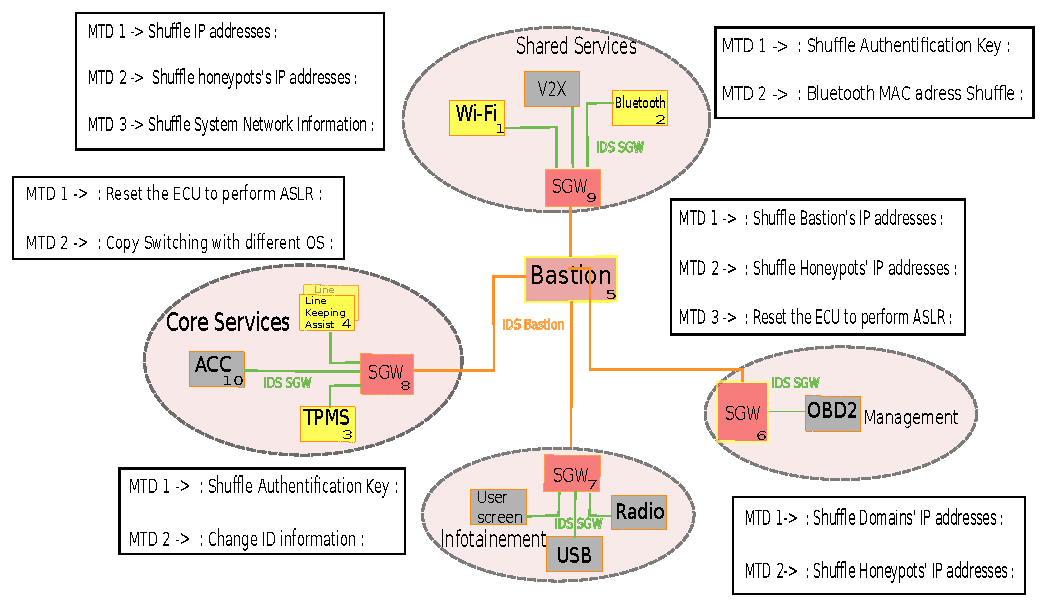
\includegraphics[width=1\textwidth]{schema/archi_comp.pdf}
    \caption{Full game representation}
    \label{fig:archi_mtd}
\end{figure}

This architecture corresponds to a game containing 10 nodes, each having between two and three MTD for defense, with ten attacker profiles taken into account when developing the strategy.
We generated the MILP corresponding to this architecture that we resolved using the CPLEX tool. We obtain the following defense strategy presented in \ref{def_strat} in which the defender will defend each node and MTD targeted by an attacker by spending its budget of 1 per node.  And the attacker strategy presented in \ref{att_strat}.
The time required to compute a solution to the problem with CPLEX is $9.2$ seconds.


\begin{align}
\delta_{n0_m0} &= 0.351 & \delta_{n0_m1} &= 0.0 & \delta_{n0_m2} &= 0.648  & \delta_{n0idl} &= 0.0 \nonumber \\
\delta_{n1_m0} &= 0.95 & \delta_{n1_m1} &= 0.05 & \delta_{n1_m2} &= 0.0 & \delta_{n1idl} &= 0.0 \nonumber  \\
\delta_{n2_m0} &= 0.0 & \delta_{n2_m1} &= 1.0 & \delta_{n2_m2} &= 0.0 & \delta_{n2idl} &= 0.0 \nonumber  \\
\delta_{n3_m0} &= 1.0  & \delta_{n3_m1} &= 0.0 & \delta_{n3_m2} &= 0.0 & \delta_{n3idl} &= 0.0 \nonumber  \\
\delta_{n4_m0} &= 0.403 & \delta_{n4_m1} &= 0.310 & \delta_{n4_m2} &= 0.285 & \delta_{n4idl} &= 0   \nonumber  \\
\delta_{n5_m0} &= 0.0 & \delta_{n5_m1} &= 1.0 &\delta_{n5_m2} &= 0.0 & \delta_{n5idl} &= 0.0  \nonumber  \\
\delta_{n6_m0} &= 0.0 & \delta_{n6_m1} &= 1.0 & \delta_{n6_m2} &= 0.0 & \delta_{n6idl} &= 0 \nonumber  \\
\delta_{n7_m0} &= 0.0 & \delta_{n7_m1} &= 0.921 & \delta_{n7_m2} &= 0.078 & \delta_{n7idl} &= 0  \nonumber  \\
\delta_{n8_m0} &= 0.0 & \delta_{n8_m1} &= 1.0 & \delta_{n8_m2} &= 0.0 & \delta_{n8idl} &= 0 \nonumber  \\
\delta_{n9_m0} &= 0.519 & \delta_{n9_m1} &= 0.480 & \delta_{n9_m2} &= 0.0 & \delta_{n9idl} &= 0 \label{def_strat} \\ \nonumber \\
\alpha_{p0_n0_m0} &= 1.0 & \alpha_{p1_n9_m1} &= 1.0 & \alpha_{p2_n4_m1} &= 1.0 & \alpha_{p3_n1_m0} &= 1.0 & \alpha_{p4_n7_m2} &= 1.0 \nonumber \\
\alpha_{p5_n0_m2} &= 1.0 & \alpha_{p6_n9_m0} &= 1.0 & \alpha_{p7_n4_m0} &= 1.0 & \alpha_{p8_n7_m1} &= 1.0 & \alpha_{p9_n1_m1} &= 1.0  \label{att_strat}
\end{align}


\subsection{Scaling tests}

\subsubsection{Random generator}

In order to investigate if the proposed solution scales well, we have generated random scenarios of different size \footnote{The generating tool we made for the experimentation is available for clone here : https://gitlab.telecom-paris.fr/TheseMA/tool\_for\_journal.git}.

During our experiments, we realized that generating the parameters in a totally random way corresponds to the worst case scenario for the defender in which all the attacker profiles are interested by all the nodes and MTD of the game. This slows down the solution search and limits the size of a game to 15 attacker profiles for 15 nodes. \\

To resolve this issue and to have a more realistic scenario generator, we limit the interest of an attacker to two thirds of the MTD present on the nodes in a random way. 

The results obtained are summarized in Figure~\ref{fig:game_pres}, in which we display the computation time taken by CPLEX to solve the problems. The scenarios are generated in such a way to have as many attacker profiles as nodes. With the parameters of the game generated randomly. This way we get an execution time for a scenario with 10 nodes and 10 attacker profiles of the same range as the one presented in \ref{expe_case}.

\begin{figure}[h]
    \centering
    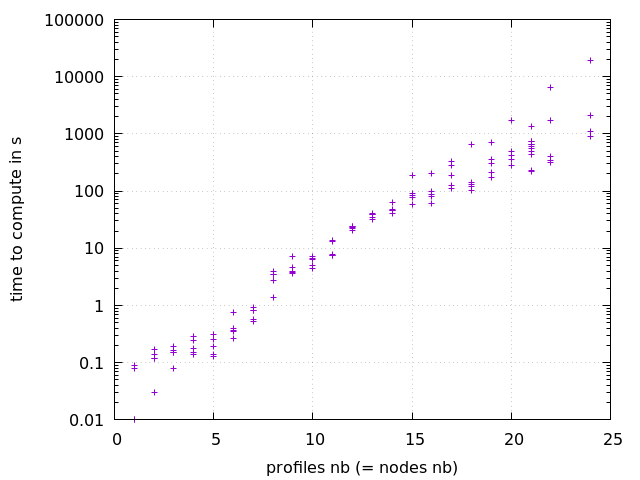
\includegraphics[width=0.75\textwidth]{schema/plot_control_log.png}
    \caption{Scaling representation with attacker profiles number = node number}
    \label{fig:game_pres}
\end{figure}


We manage to reach reasonable times with games composed of 25 nodes and 25 attacker profiles.

An automotive system is made up of an average of a hundred assets that we will try to protect, this amounts to about 25 nodes per domain.

If we consider that the game corresponds to the strategy to be defined on a domain, this is not disadvantageous on the attacker's side, who finds himself attacking each domain once. On the defender's side it does not change anything in the principle of finding the strategy.

\subsubsection{Fixed attacker profiles generator}

In a realistic scenario, it is more common to choose a fixed number of attacker profiles defined in advance according to the type of identified attack scenario being considered.

We can look for the best possible strategy by considering that there will only be privacy attackers interested by the vehicle, and that among these types of attackers, there will be 5 levels of expertise taken into account expert/high/medium/low/beginner. 

If we now consider that we have privacy and integrity attackers targeting the system, with 5 levels of expertise each, we arrive at 10 attacker profiles to take into account in the game.

In the case we want to be even more precise and we know 10 specific attackers trying to attack us in addition to the 10 profiles previously taken into account, we arrive at 20 attacker profiles. \\

We wanted to check up to how many nodes we could consider in order to find a solution, this is represented on the figure~\ref{fig:full}. 
As can be noticed, there are no scenarios where the number of nodes is smaller than the number of attacker profiles considered. This is due to the form of our model in which the attacker has a global budget for the game while the defender has one budget per node. This leads to an infeasibility of the problem because of constraints \ref{c1_milp}, \ref{c3_milp} and \ref{c4_milp} of the MILP. \\

\begin{figure}[h]
    \centering
    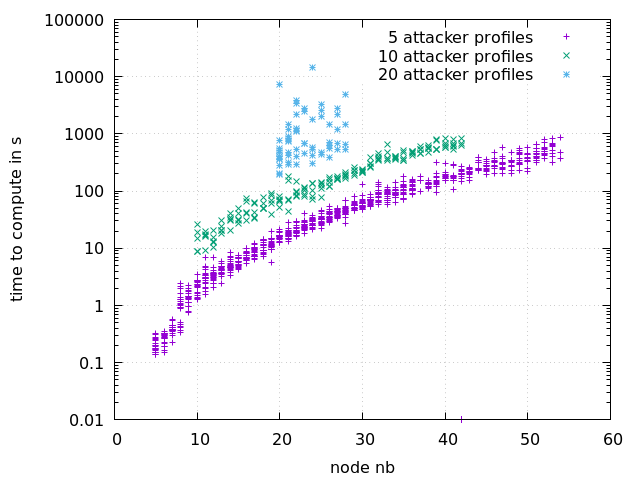
\includegraphics[width=0.75\textwidth]{schema/plot_cplex.png}
    \caption{Scaling representation with fixed attacker number profiles and increasing node number}
    \label{fig:full}
\end{figure}


By looking at the results of the scaling test with different types of attacker profiles considered, we notice that by taking into account 1 type of attacker (5 profiles), it is possible to scale up to 55 nodes with 3 different MTD each. On systems where only one type of attacker is considered, this type of model allows to calculate a strategy for the defender in a reasonable time.

For systems in which 2 types of attackers are taken into account (10 profiles), it is possible to find a solution in a reasonable time for 40 nodes each having 3 MTD. This corresponds to finding a strategy for a domain of a car-like system. 

On the other hand, for systems taking into account a larger number of attacker profiles (20 profiles), we are limited to 30 nodes to find a strategy in a reasonable time. This becomes complicated for automotive systems.

\subsection{Stability Analysis}

We realized a stability analysis on different parameters of our game. As it is difficult to characterize some parameters, we wanted to increase the confidence we have in our model in case of an approximation error in the definition of some parameters such as the rate of appearance of an attacker profile, or the cost of an attack for an attacker. \\

We therefore started with the parameter $\gamma$ representing the rate of appearance of an attacker profile. We then varied the ratio between the two types of attackers (privacy and integrity) for a lambda configuration of their exponential distribution in order to see the impact that this would have on the defender's strategy. We started with a configuration of the game similar to the one presented in the example case, 10 nodes each having between 2 and 3 MTD being targeted by 10 attacker profiles.
The results of this experiment for 4 of the nodes in our game are presented in figure \ref{fig:gamma}. \\

\begin{figure}[h]
    \centering
    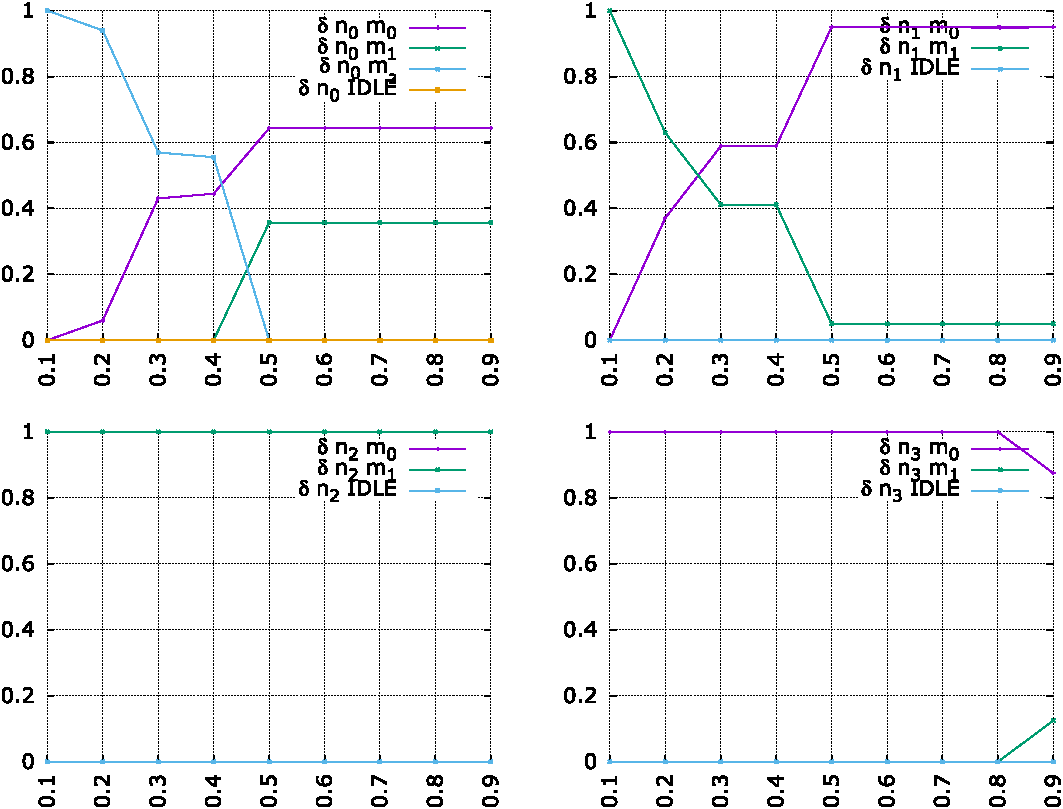
\includegraphics[width=1\textwidth]{schema/multiplot_gamma.pdf}
    \caption{How moving the ratio between attacker profiles (gamma) affect the defender strategy}
    \label{fig:gamma}
\end{figure}


We notice that the variation is linear, and that the defender's strategy reacts in a normal way to the change of ratio between the attackers.
On a node like number 0 and 1 on which more attacker profiles target them, depending on the ratio of attacker profile, the strategy evolves in order to defend more efficiently against the type of attacker becoming more present.

On nodes such as node number 2, targeted by no attacker type, this does not change the strategy of the defender, and on the fourth node, when the ratio of the second attacker type becomes more present, the strategy of the defender starts to adapt. \\


In order to then look at the stability of the given strategy according to a set of input parameters, we sum of a fixed scenario using the configuration of the example case. Then we randomly shuffled the value of the costs and gain for the defender and the attacker as well as the attacker success value of the scenario around a certain percentage of variance in order to check the stability of the output strategy. The result of this variance is represented in figure \ref{fig:multiplot} with box plot representing the variation of strategy of the defender on 100 different scenario. 

\begin{figure}[h]
    \centering
    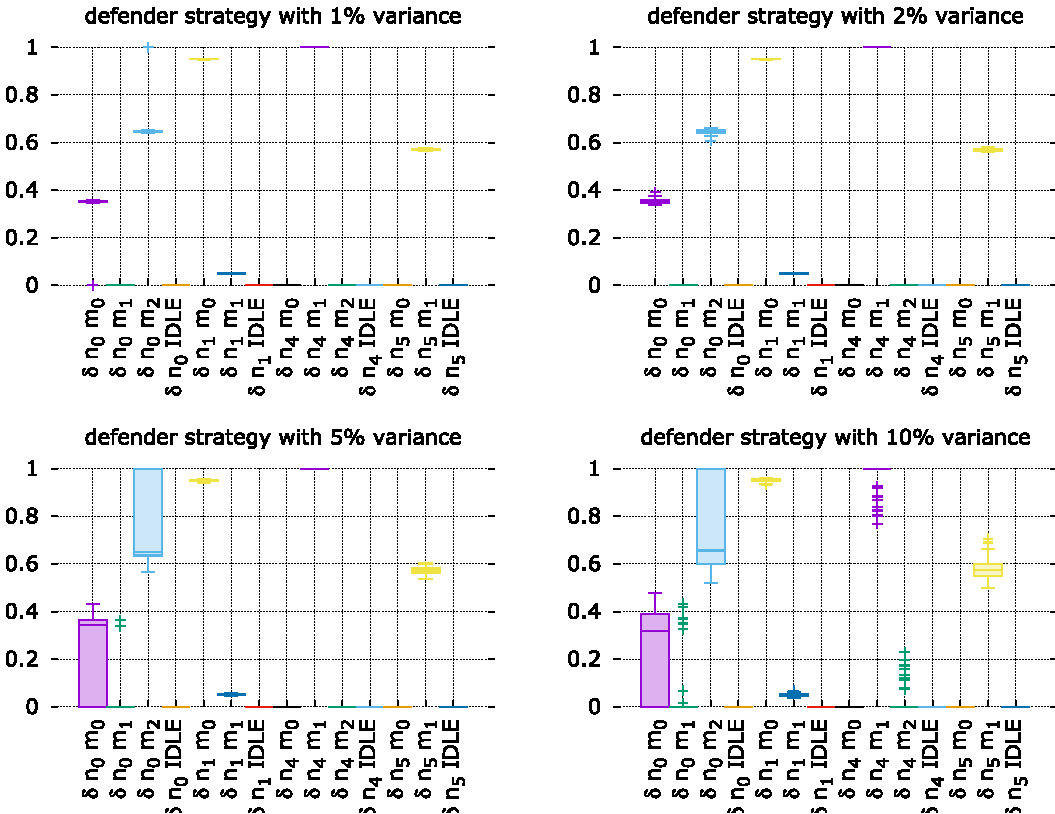
\includegraphics[width=1.0\textwidth]{schema/multiplot.pdf}
    \caption{How stable the strategies are considering variance in the parameters}
    \label{fig:multiplot}
\end{figure}

We also notice that the strategy variation remains quite stable up to 5\%. At this moment, on the node 0 where the balance between the two attackers is borderline, we notice a change of strategy. But we notice that the medians of the strategies on this node are still located in the same order of magnitude, indicating that the strategy remains mostly located in the same area.
From 10\% we start to notice a more important variance in the strategy of the defender, with an average strategy always located in the same region.
We can say that our model reacts in a normal way to the variations in the parameters and is quite stable allowing us to have confidence in the final strategy taking into account a small possible margin of error in the definition of the parameters.
